\documentclass[10pt,journal]{IEEETran}
\usepackage{amsmath}
\usepackage{graphicx}
\usepackage{float}
\usepackage{algorithmic}
\usepackage{algorithm}
\usepackage{enumitem}
\title{Haar Cascade Classifiers for Hand Gesture Recognition}
\author{Ronit Rudra \\Department of Computer Science\\Illinois Institute of Technology\\rrudra@hawk.iit.edu\\A20379221 \\ Prerna Kapoor\\Department of Computer Science\\Illinois Institute of Technology\\pkapoor1@hawk.iit.edu\\A20371648}
\begin{document}
\maketitle
\begin{abstract}
This paper proposes the design and development of a program that is capable of recognizing multiple hand gestures using multiple Haar Cascade Classifiers. Gesture recognition is an important tool in the field of Human Computer Interaction. These machines can understand instructions through user?s face, voice, hand movements etc. Gesture recognition can be seen as a way for computers to begin to understand human�body language, thus building a richer bridge between machines and humans than primitive�text user interfaces�or even�GUIs�(graphical user interfaces), which still limit the majority of input to keyboard and mouse. [1] In this project we detect multiple hand gestures and once these gesture are detected, we trigger events based on these gestures. Hand gesture recognition is done through computer vision and machine learning algorithms. Hand-pose detectors are trained with a reduced Haar-like feature set and the AdaBoost learning algorithm to make the detector robust. Then region of interest is extracted from the detected hand and convex hull algorithm is applied to the image. Thus, multiple hand gestures are recognized in real time.
\end{abstract}
\begin{IEEEkeywords}
Haar Cascade, Background Subtraction, Skin Color Detection, Supervised Learning, Feature Engineering.
\end{IEEEkeywords}
\section{Problem Statement}
The objective is to recognize a hand gesture from the complete frame in the video. Then, the program should detect either of the \textbf{3 gestures} ? if it is a "Palm", "One Finger" or "Two fingers". The program should then perform tasks based on different features such as "Open Textedit", "Open Google Chrome" or "Open Word" respectively.
\section{Proposed Solution}
There are several steps involved in the gesture recognition such as data collection, preprocessing, creating positive and negative images, training Haar features, finding convex hull based on the region of interest detected by the classifier. Each of the steps are explained below:
\subsection{Haar Cascade}
This is the most important aspect of the project. Haar is a machine learning based approach where a cascade function is trained from a lot of positive and negative images. It is then used to detect objects in other images. [4] The concept of Haar training begins with positive and negative images. Positive images are the ones which contain the object(hand gesture) and negative images are random images which do not contain the object. Haar training occurs using multiple stages on a large set of positive and negative images and a cascase is created for each stage. There is a final cascade created which is the combination of all the stages. Once the training is finished then, we can test the code real time. Thus, we train Haar differently for all the gestures and thus we can detect if it is a "palm" or "one finger" or "two fingers" shown by the user.
\subsection{Background Subtraction}
Another step in preprocessing the frame in the video is to detect the hand. Background subtraction, also known as�foreground detection, is a technique in the fields of�image processing�and�computer vision�wherein an image's foreground is extracted for further processing. Generally an image's regions of interest are objects (humans, cars, text etc.)
in its foreground. In this case, a hand is our object of interest. There are several applications for background subtraction.�For example, consider the cases like visitor counter where a static camera takes the number of visitors entering or leaving the room, or a traffic camera extracting information about the vehicles etc. In all these cases, first you need to extract the person or vehicles alone.
\par There are 2 ways to calculate the background subtraction ? Firstly if we have an image of just the background and then another image of the foreground object(or hand) then we can easily subtract the new image from the background image but in real time applications most of the time this is not the case. Thus, we need to extract the foreground
from the images. As shown in the images above, the hand is captured as foreground.
\subsection{Skin Color Detection}
The first step in preprocessing in Skin Color Detection. So, we select skin-color to get characteristics of hand. The skin-color is a distinctive cue of hands and it is invariant to scale and rotation. Human Skin detection deals with the recognition of skin-colored pixels and regions in a given image. The three main parameters for recognizing a skin
pixel are HSV (Hue, Saturation, Value) and YCbCr (Luminance, Chrominance) color models as the components are orthogonal to each other and the color is independent of the illumination. Once the binary image is obtained we apply different levels of morphological operations such as erosion and dilation This operation consists of convoluting an image�with some kernel.
\begin{enumerate}
\item \textit{Dilation:} As the kernel�is scanned over the image, we compute the maximal pixel value overlapped by�the kernel�and replace the image pixel in the anchor point position with that maximal value. As you can deduce, this maximizing operation causes bright regions within an image to "grow".
\item \textit {Erosion:} This operation is the sister of dilation. What this does is to compute a local minimum over the area of the kernel. As the kernel�is scanned over the image, we compute the minimal pixel value overlapped by��and replace the image pixel under the anchor point with that minimal value. In this case the brighter parts of an image get
smaller.
\end{enumerate}
\subsection{Convex Hull}
Convex hull builds the smallest polygon, which can wrap all the contours. Contours can be explained simply as a curve joining all the continuous points (along the boundary), having same color or intensity. The contours are a useful tool for shape analysis and object detection and recognition. This is the last stage and is used for visualization and backup detection.
\begin{figure}[H]
\centering
\caption{Convex Hull}
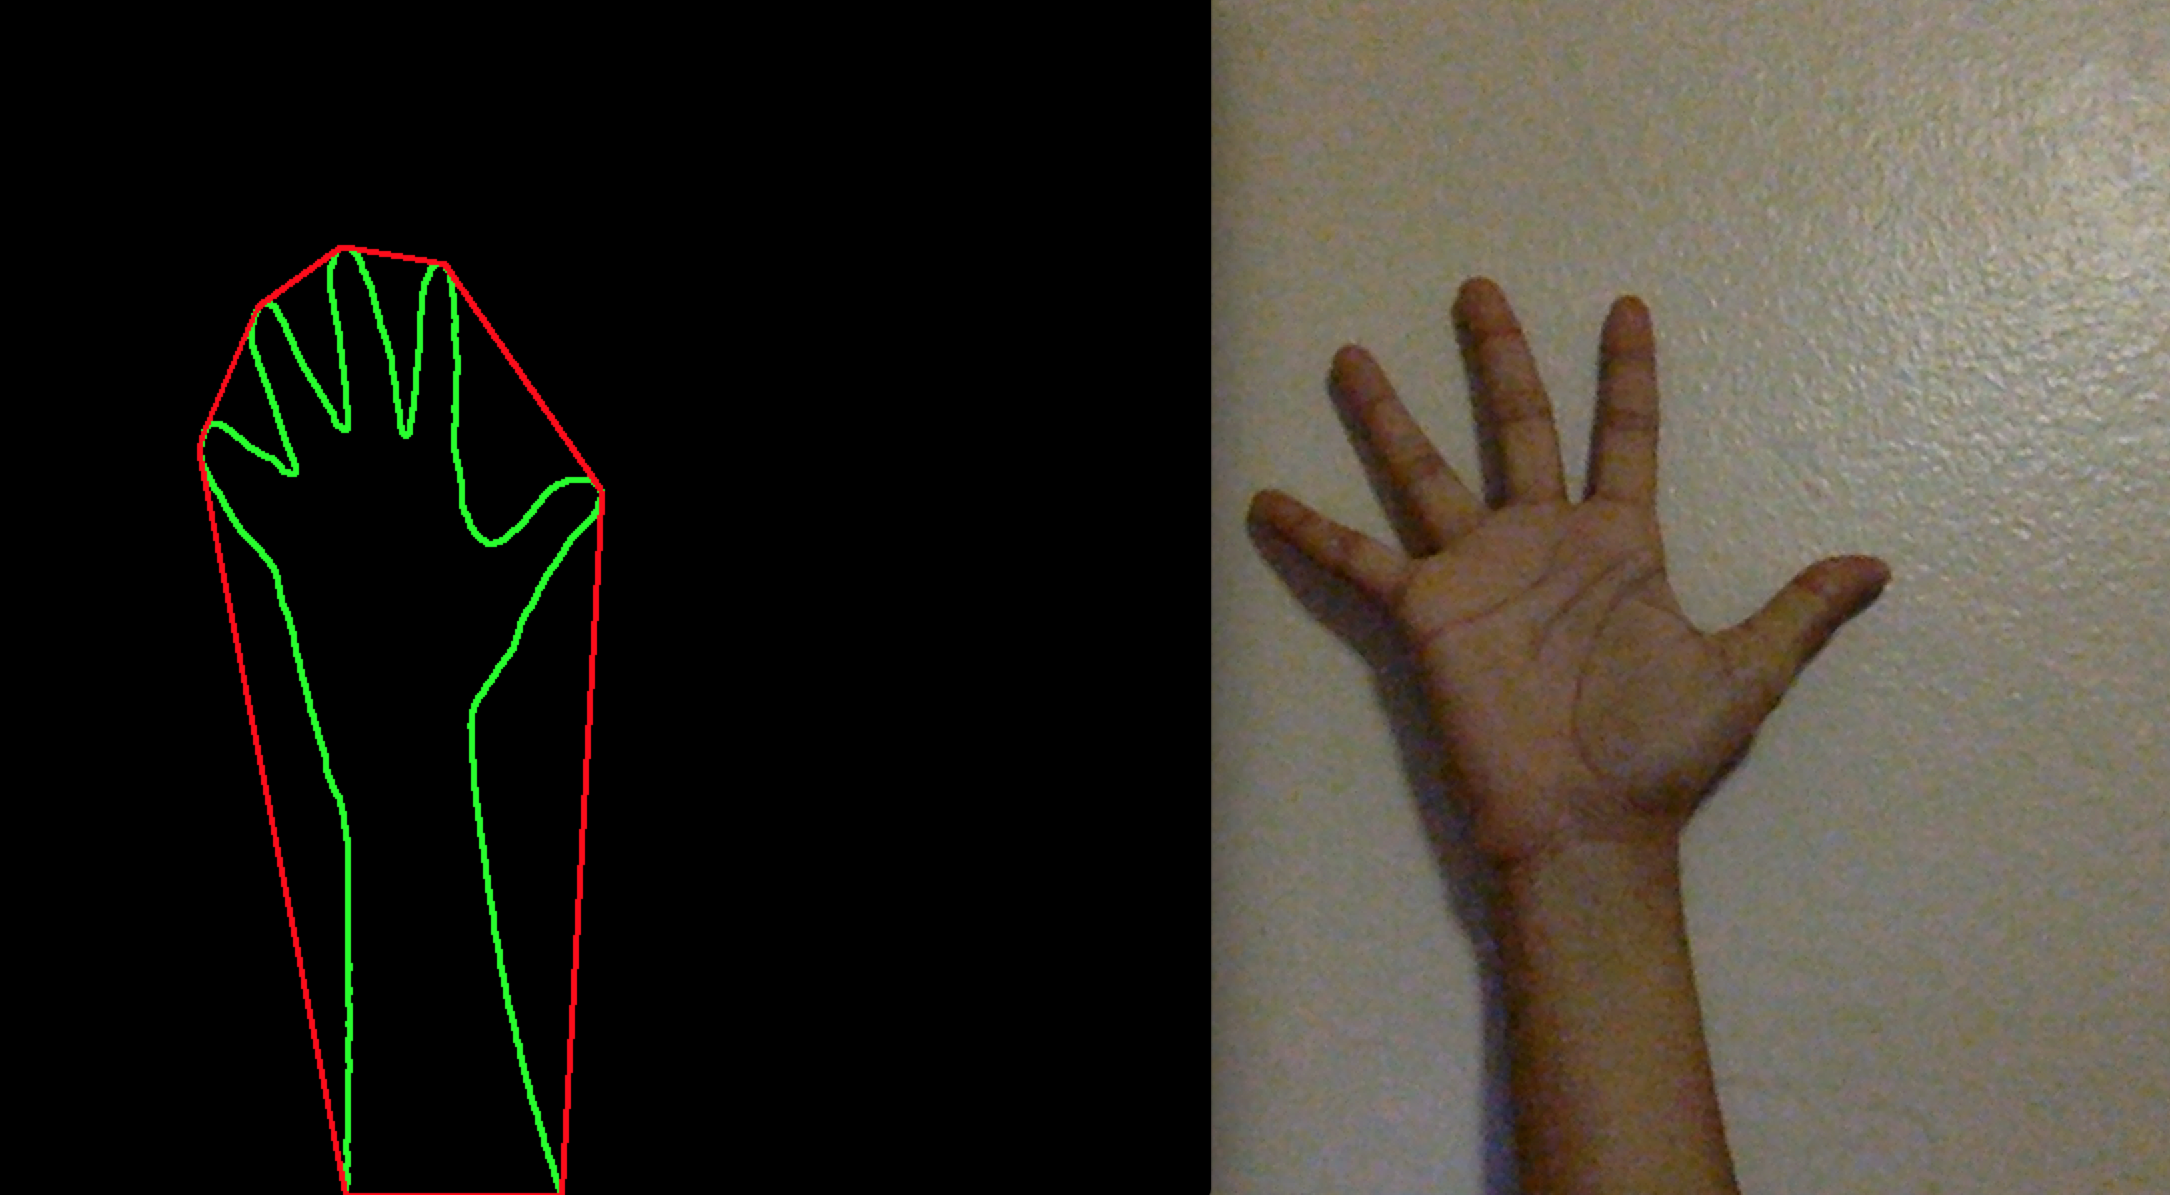
\includegraphics[width=8cm,height=4cm,angle=0]{convex_hull}
\end{figure}

%% DO NOT MAKE CHANGES BELOW THIS LINE
%%=============================================================================================================================================================================
\section{Implementation Details}
This section describes the implementation of the cascade detector including the data collection and preprocessing stages. Since the Haar Cascade training is highly sensitive to the quality of inputs provided to it, the data preprocessing stage is of paramount importance. The consequences of feeding poorly preprocessed training data to the classifier is discussed in the testing section.
\par Before delving into the details there are a few definitions that should be known:
\begin{enumerate}
\item \textit{Precursor} Image containing only the object of interest. The Object is the foreground while the background is of a uniform color. The Object fills the entire image.
\item \textit{Negative Sample} Any image not containing the object of interest.
\item \textit{Positive Sample} An image constructed using the Precursor and Negative Sample by placing an affine transformed Precursor on the Negative Sample.
\item \textit{Descriptor} A string specifying the file path and description of a sample. For positives the description contains the location of the positive precursor. For negatives the description is empty. A collection of descriptors is stored in a descriptor text file.
\item \textit{vector} A \textit{.vec} file passed as an argument to the trainer. This file contains information about the positive and negative samples used in training as well as specific configurations for the trainer.
\end{enumerate}
\subsection{Data Collection}
As explained above, the data collection stage is the most important stage as feeding garbage inputs to the classifier would result in a poorly trained classifier. Therefore, a few things to keep in mind are:
\begin{enumerate}
\item Only a handful of precursor images for positive sample generation are required. Hence, the samples should be distinct from one another.
\item For gesture recognition, the hand gestures should be upright. Hence, rotation invariance is not required.
\item The negatives should be of a larger size than the positive precursors.
\end{enumerate}
\begin{enumerate}
\item \textit{Precursor Data:} Collected data using webcam (resolution of 1280x720) for 3 different gestures. Namely Palm, Single Finger(Index pointing up) and Two fingers (Index and Middle finger in V-Shape). 
\par A python script was used to extract the hand foreground in the ROI and label them accordingly. For each gesture, around 30 distinct images were collected. A low number of precursor positive samples is needed as the subsequent stage of the training generates thousands of positive samples from the precursors. These images were RGB with a resolution of 400x400 and were taken against an approximate uniform background in order to facilitate foreground extraction.
\begin{figure}[H]
\centering
\caption{Precursor Images}
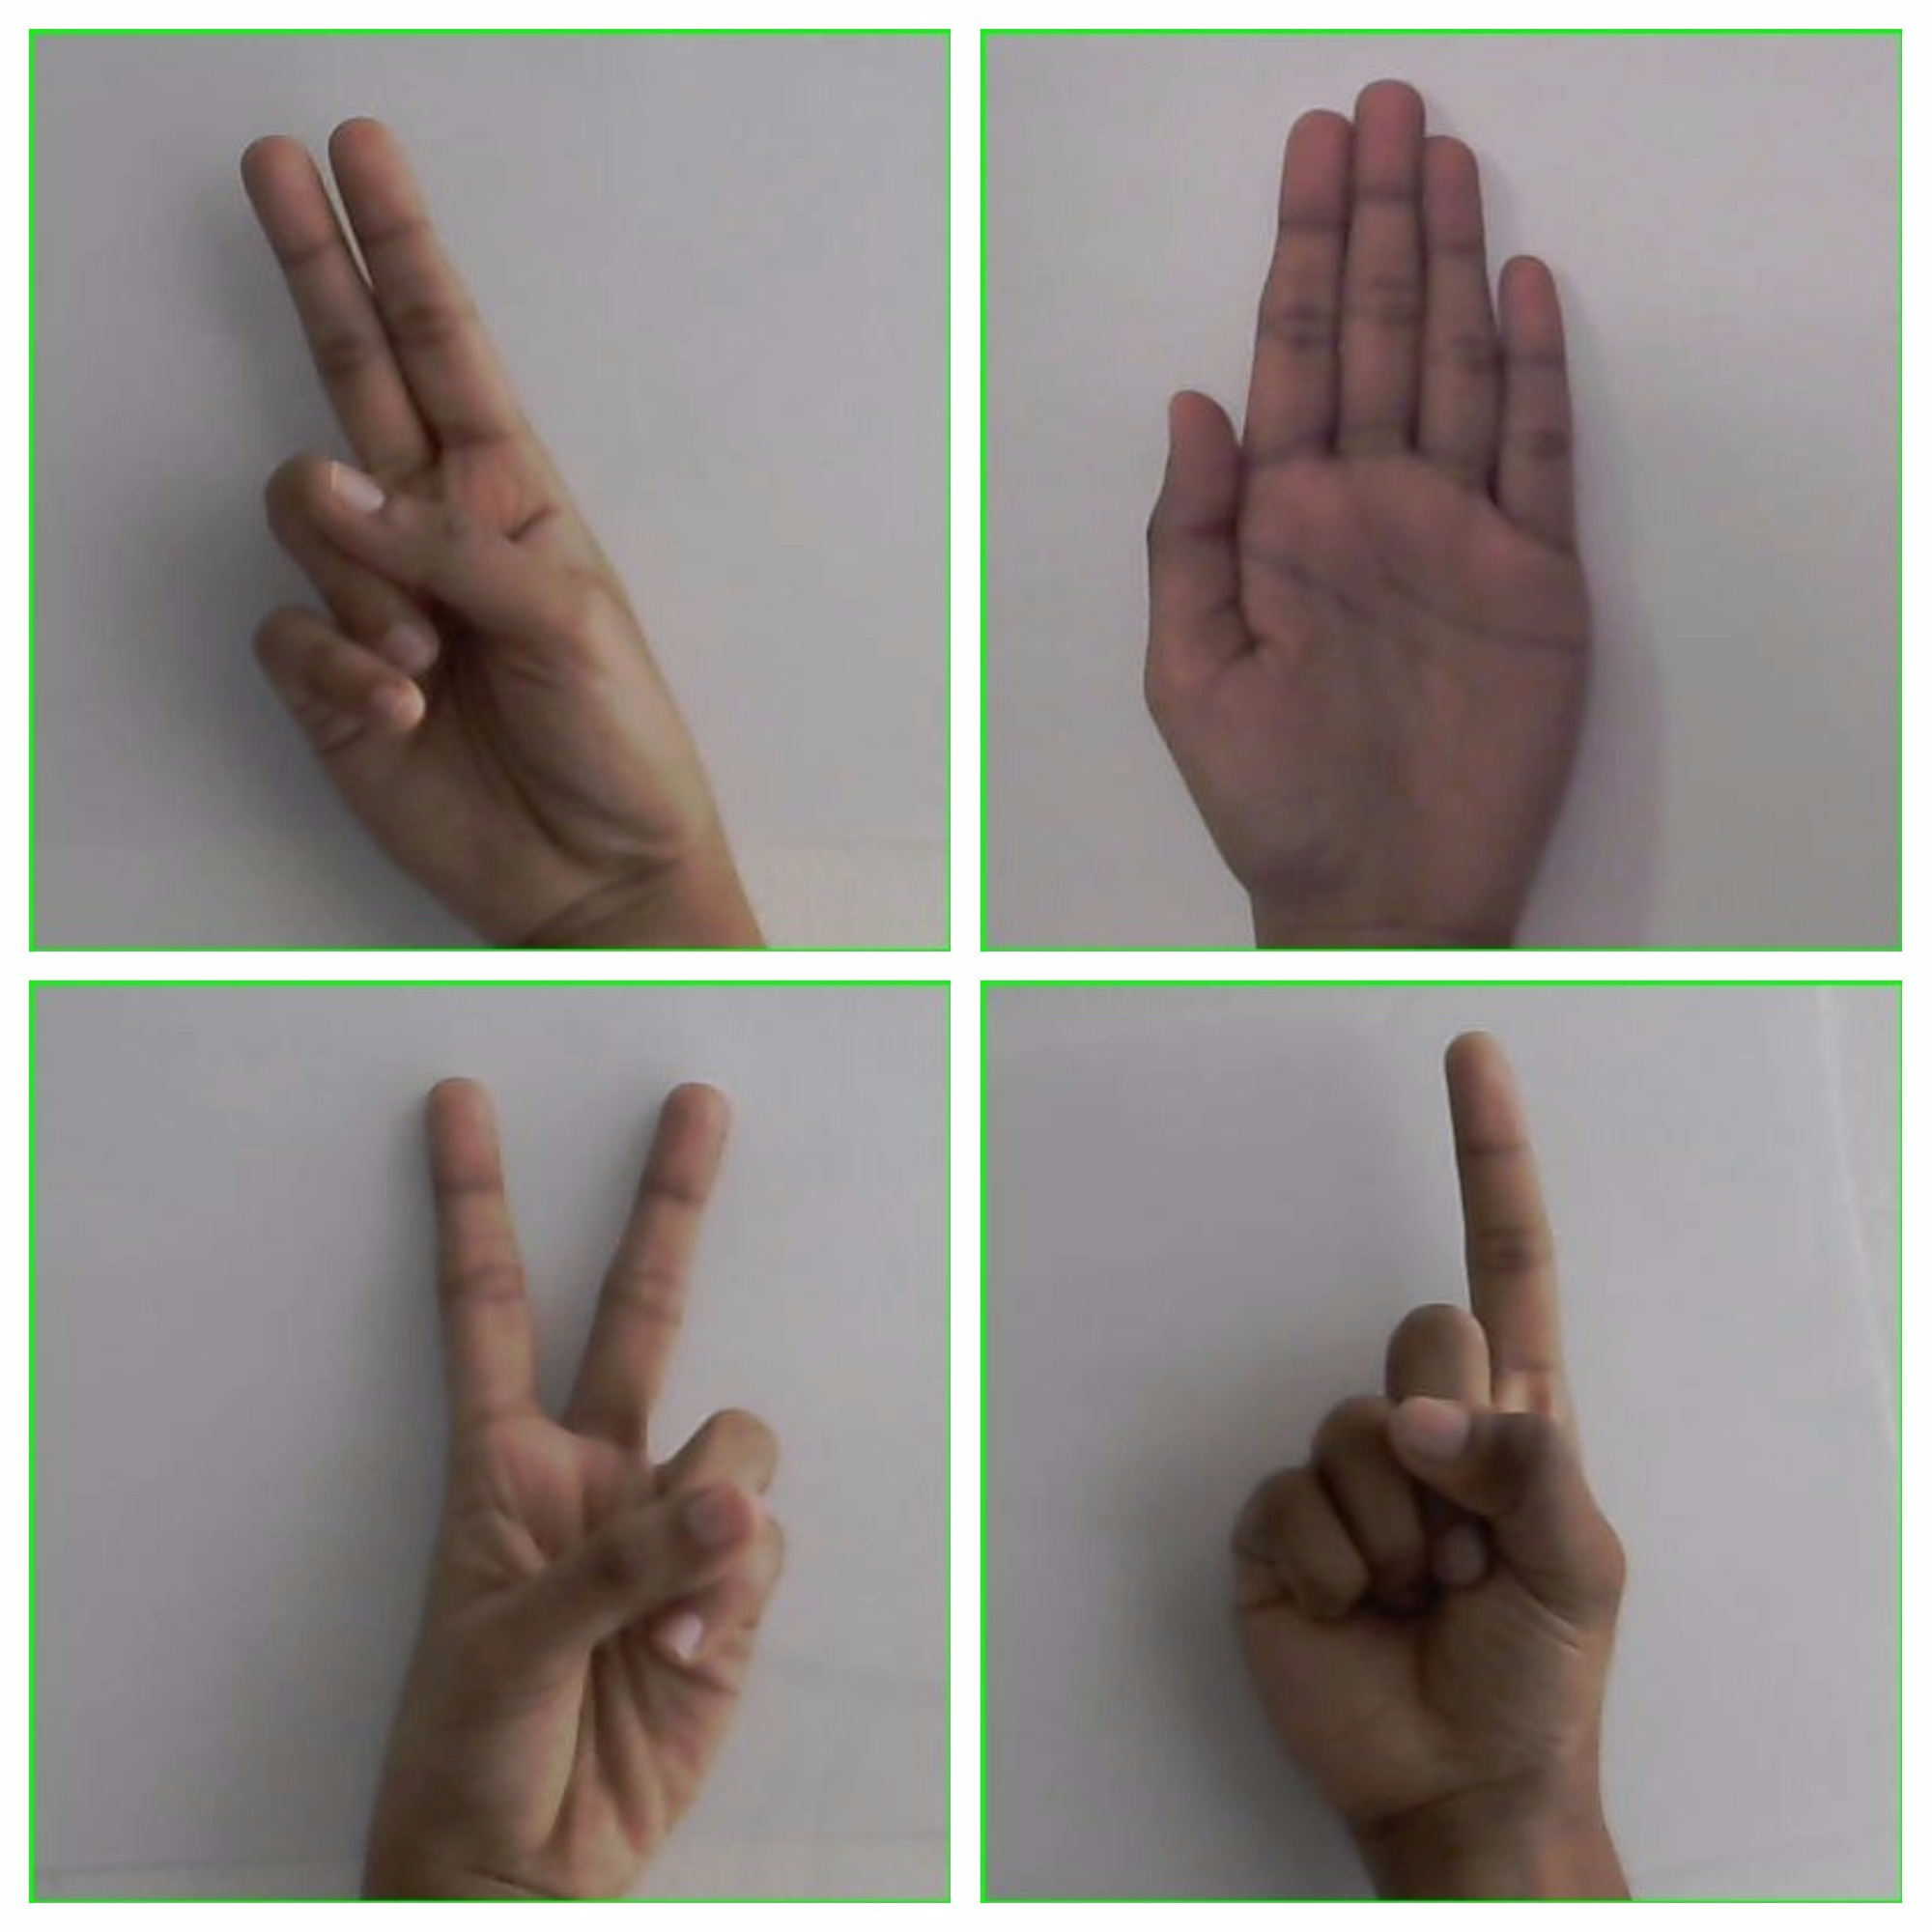
\includegraphics[width=8cm,height=4cm,angle=0]{precursor}
\end{figure}
\par For use in training, a large number of negative images were also created. Each image is grayscale with a resolution of 640x480 (The negatives need to be larger than the precursors). The negatives need to be highly detailed with a lot of clutter so that the Haar Cascade can better distinguish noise from actual features. The images used are available at [cite page].
\begin{figure}[H]
\centering
\caption{Negative Images}
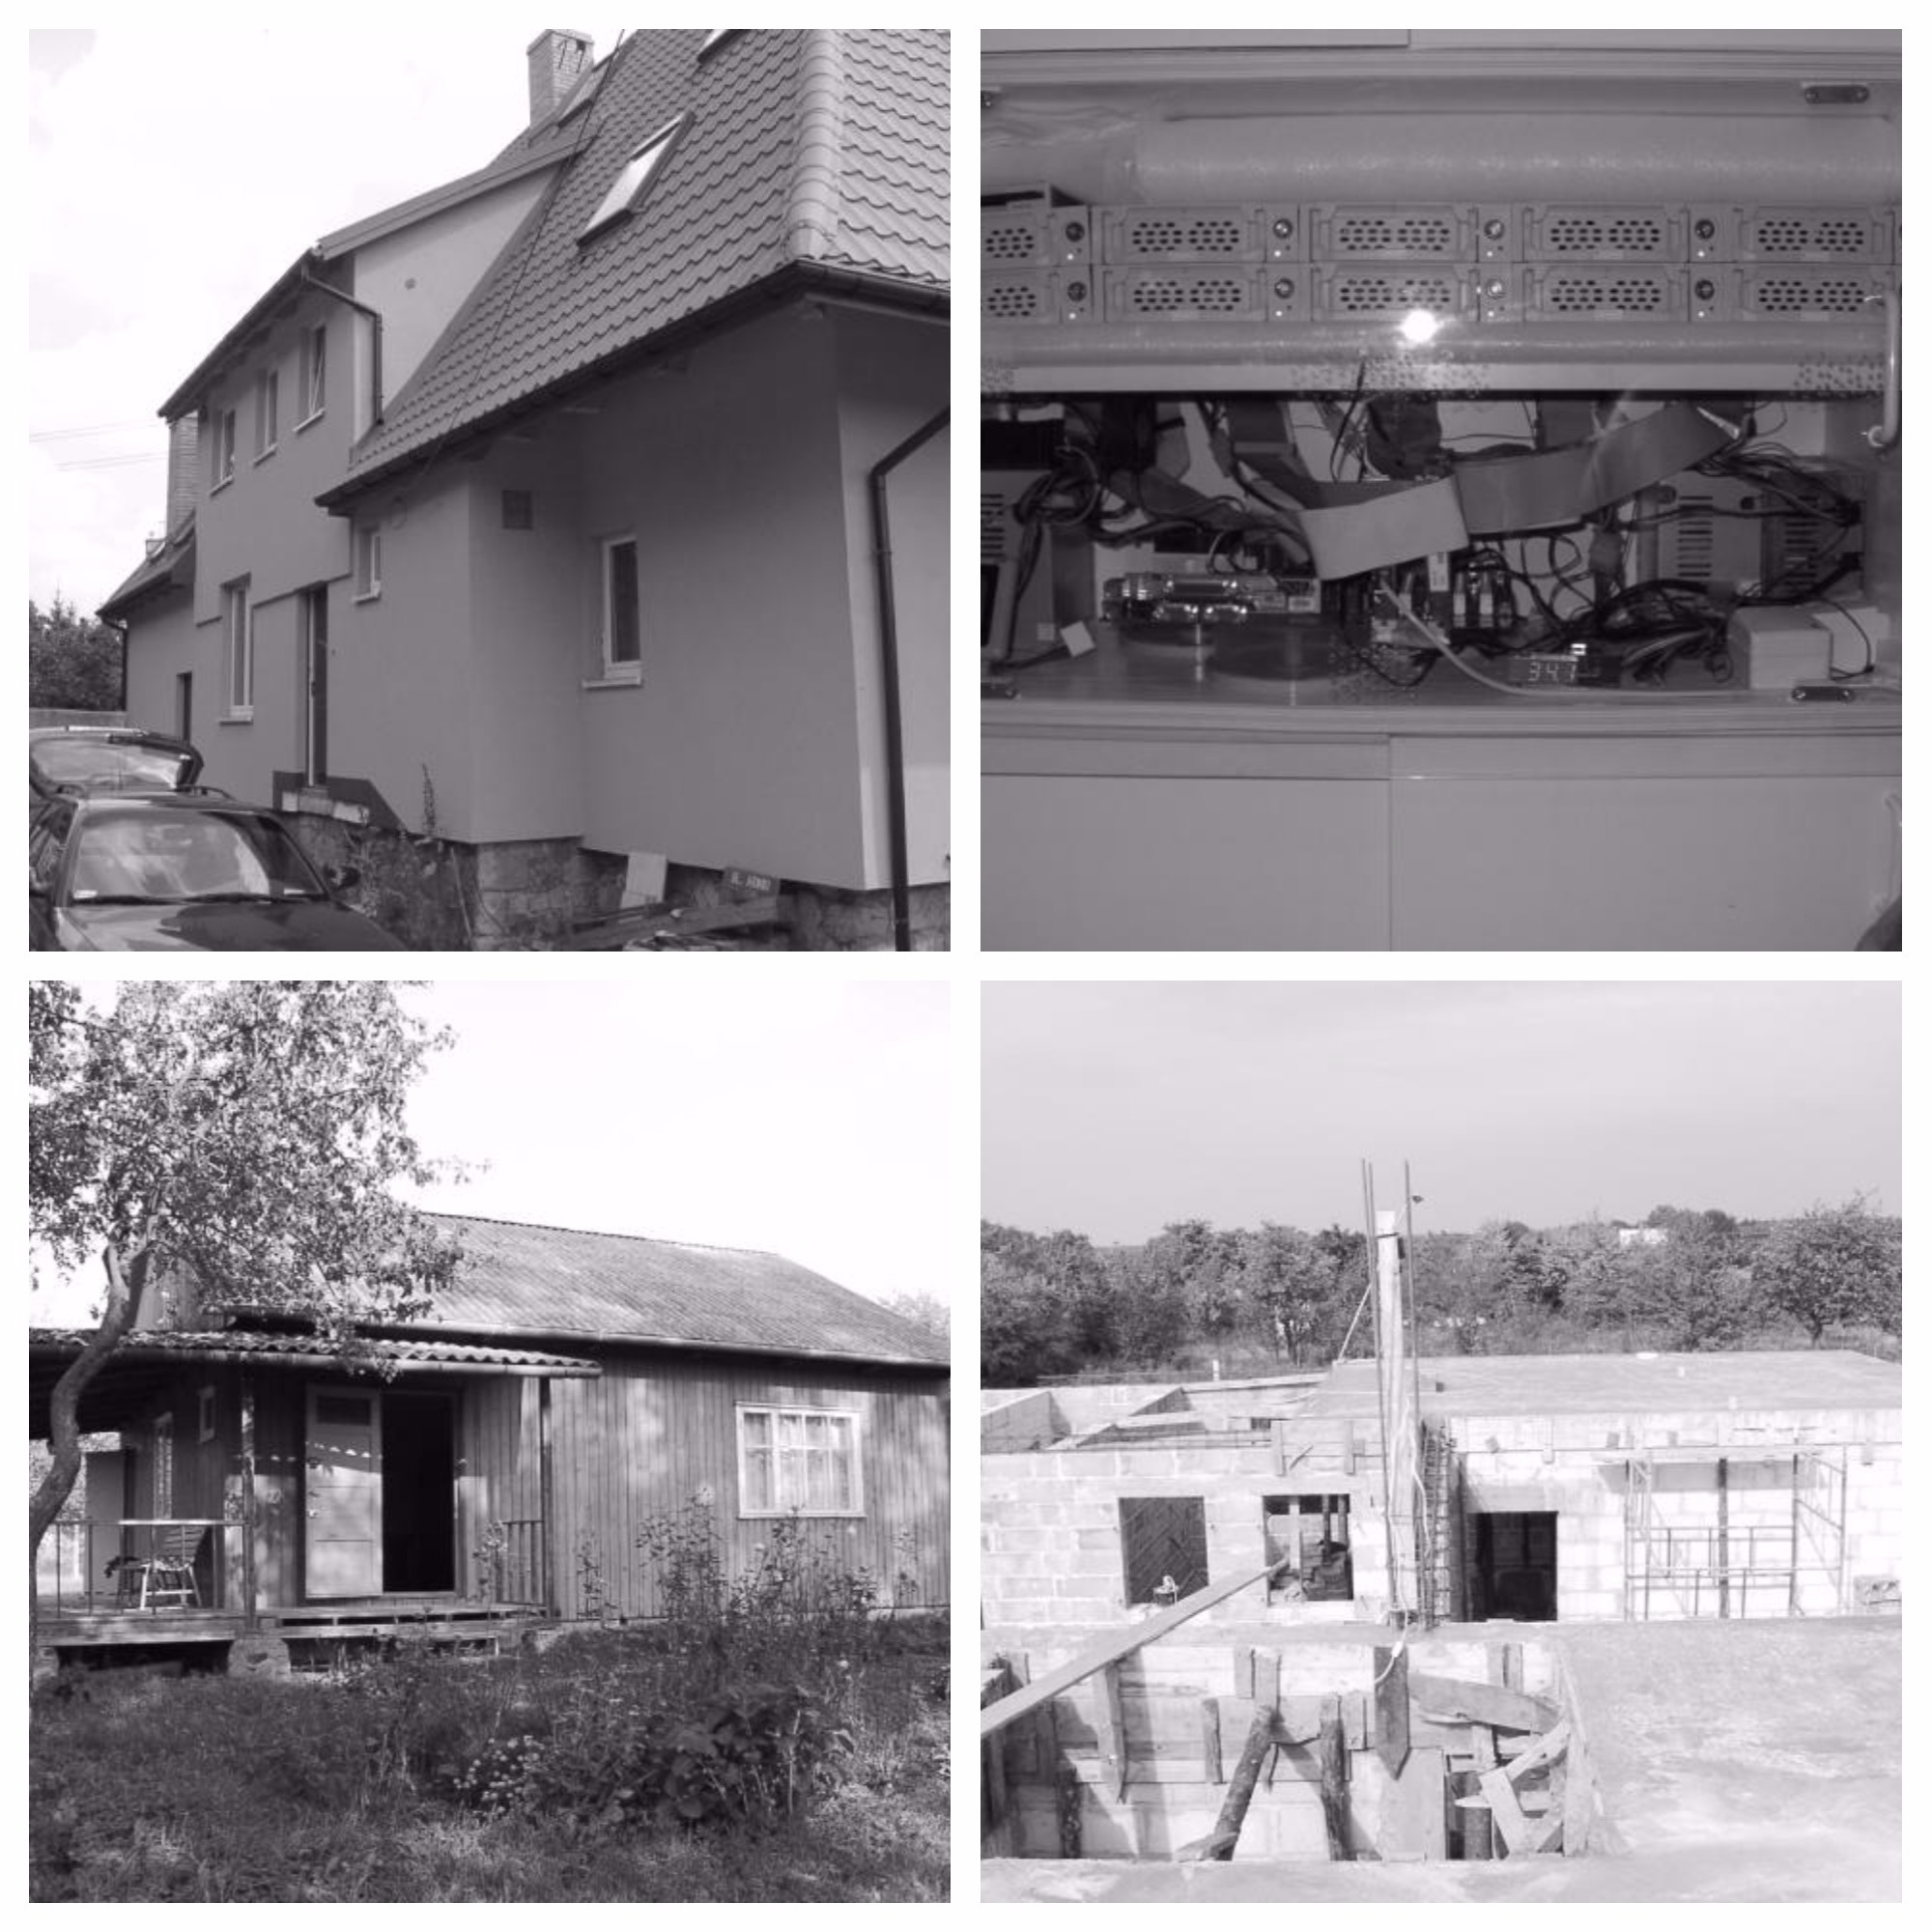
\includegraphics[width=8cm,height=4cm,angle=0]{negatives}
\end{figure}
\item \textit{Preprocessing:} The collected images were then subject to skin color detection and thresholding to obtain only the hand gesture with a white background. A white background (or any other uniform color) is necessary for the subsequent step of generating positive samples as the generator can make the background transparent. 
\par The threshold values used have been empirically estimated [cite paper]. After obtaining the binary image of the foreground by applying threshold, multiple iterations of erosion and dilation are applied to obtain a single contour of the foreground. The burned image is finally obtained by performing a \textit{Bitwise AND} with the original image to extract the hand foreground. The algorithm for obtaining the burned (only foreground) precursors is as follows:
\begin{algorithm}[H]
\caption{Foreground Extraction}
\begin{algorithmic}[1]
\STATE $I \gets$ All Input Precursors in BGR Color Space
\STATE $t_1,t_2,t_3,t_4\gets$ Threshold Ranges for $C_b$ and $C_r$ respectively
  \FORALL{$i \in I$}
	\STATE $i_c \gets$ Color Space conversion of $i$ to $YC_bC_r$ Space
	\STATE $i_t\gets$ Threshold($i_c,t_1,t_2,t_3,t_4$)
	\STATE $i_{mask}\gets$ $N$ Erosion and $M$ Dilation on $i_m$
	\STATE $i_{burned}\gets$ Bitwise AND of $i$ and $i_{mask}$
  \ENDFOR
\end{algorithmic}
\end{algorithm}
\par The above algorithm is not always accurate, so manual preprocessing is also performed on the precursors.
\begin{figure}[H]
\centering
\caption{Burned Images}
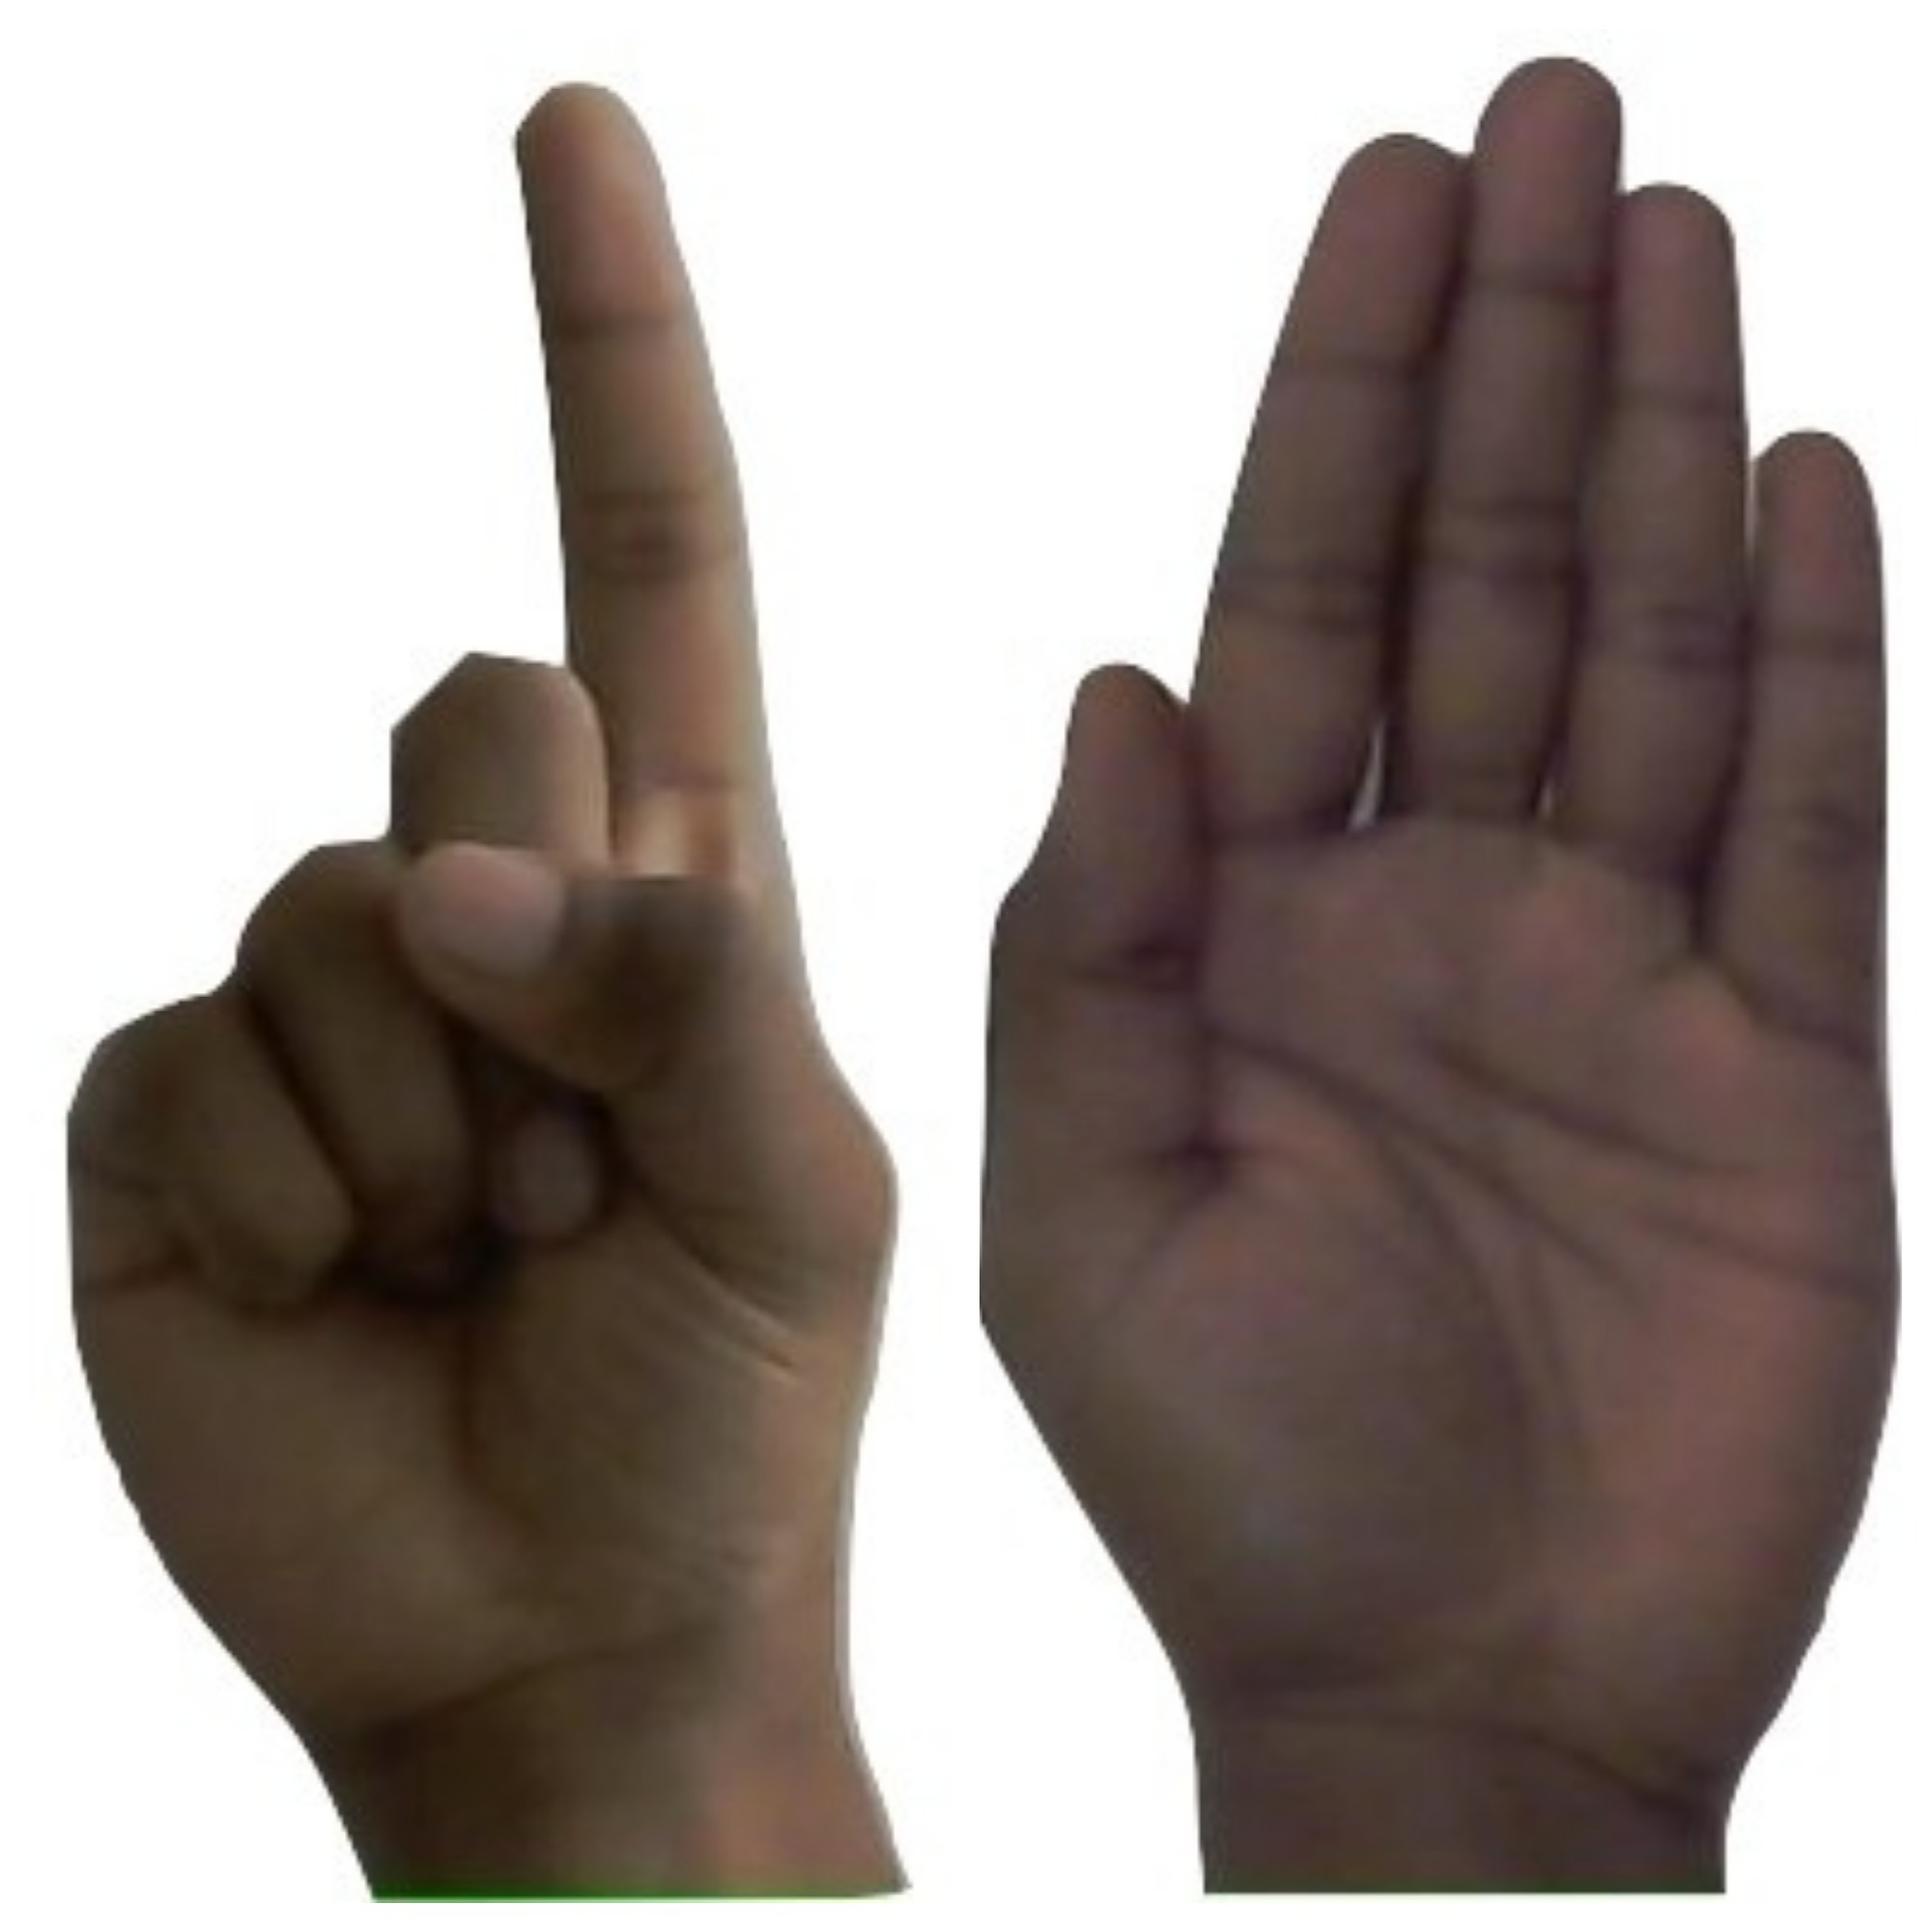
\includegraphics[width=8cm,height=6cm,angle=0]{burned}
\end{figure}
\end{enumerate}
\subsection{Training the Haar Cascades}
Training the Haar Cascade classifier is straightforward as long as the training data has been set up properly. There are two commands included in the \textit{OpenCV command line utilities}. These commands run directly from a Windows Command Line or Linux/MacOS Terminal and are much faster than python as the backend is completely in C++ and FORTRAN. The two commands used for setting up the training data and training the Haar Cascade are \textbf{opencv\_createsamples} and \textbf{opencv\_traincascade}.\par
For our purposes, we trained three distinct classifiers, one for each gesture. There were two different classifiers for each gesture as below:
\begin{enumerate}
\item \textit{Vanilla Negatives} The negative samples were the original samples gathered from [cite page].
\item \textit{Augmented Negatives} The negatives were the positives for the other gestures. For example, when training the two finger gesture, the positive images of the open palm and one finger gestures were used as negatives.
\end{enumerate}
\par The Working Directory is to be set up before the training can take place. The directory should be exact since the process flow assumes the required files to be in the correct sub-directories. The root directory should contain the sub-directories: \textit{neg, pos, info, data}.
\par The following parts assume that the training is taking place for a single gesture. This is repeated for the other gestures as required.
\begin{enumerate}
\item \textit{Negative samples:} Negative samples are first collected and placed in the \textit{neg} subdirectory. The negative samples are used to generate a descriptor file (stored in root) which points to the locations of all the negative images. This would be used in training as well as for generating positive samples.
[image of negative descriptors]
\item \textit{Positive samples:} The command \textit{opencv\_createsamples} is run iteratively on each of the precursors. this creates a large number of positive images from one precursor image by placing an affine transformed (scale, translation, rotation, skew) image of the precursor on randomly chosen negative images. The output is stored in the \textit{info} subdirectory. The negative sample descriptor file is used as an index for locating the negative samples. This also generates a descriptor file specifying the filename and the location of the object of interest (in our case the hand gesture) in the image. These descriptors would be used in generation of a vector file for use in training.
\begin{figure}[H]
\centering
\caption{Positive Images}
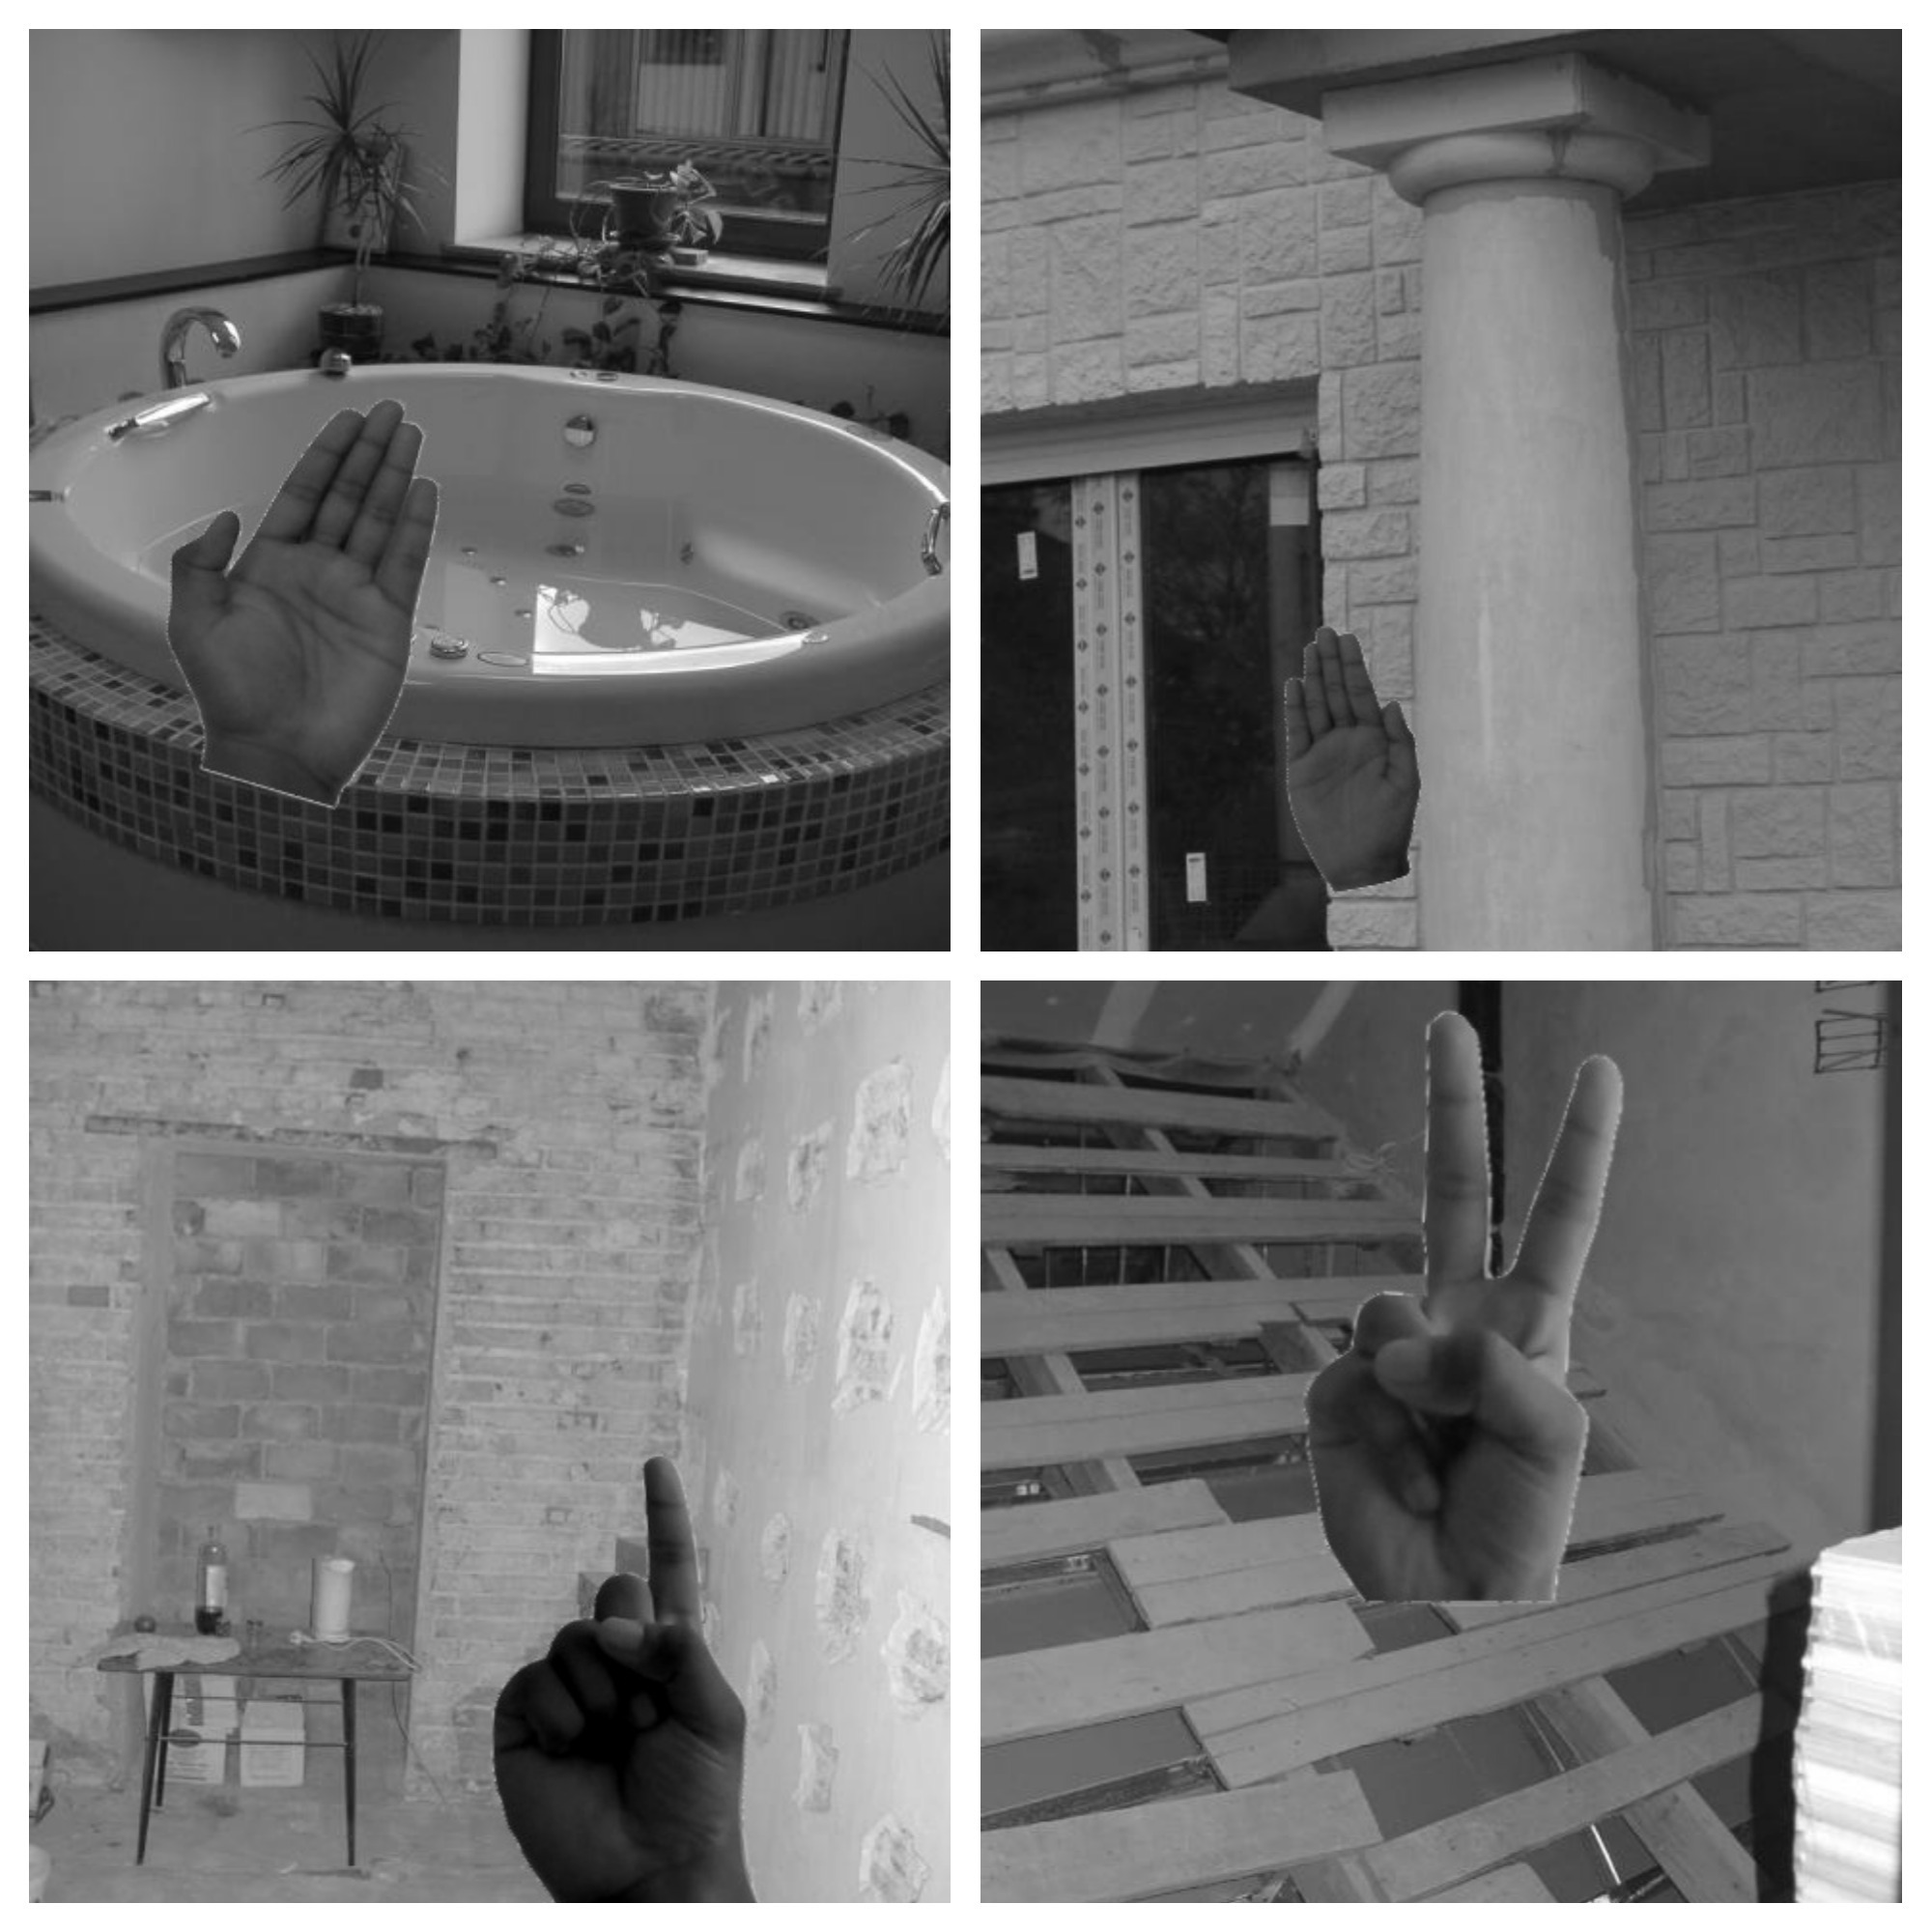
\includegraphics[width=8cm,height=4cm,angle=0]{positive}
\end{figure}
\begin{figure}[H]
\centering
\caption{Augmented Positives for 2 Finger Gesture}
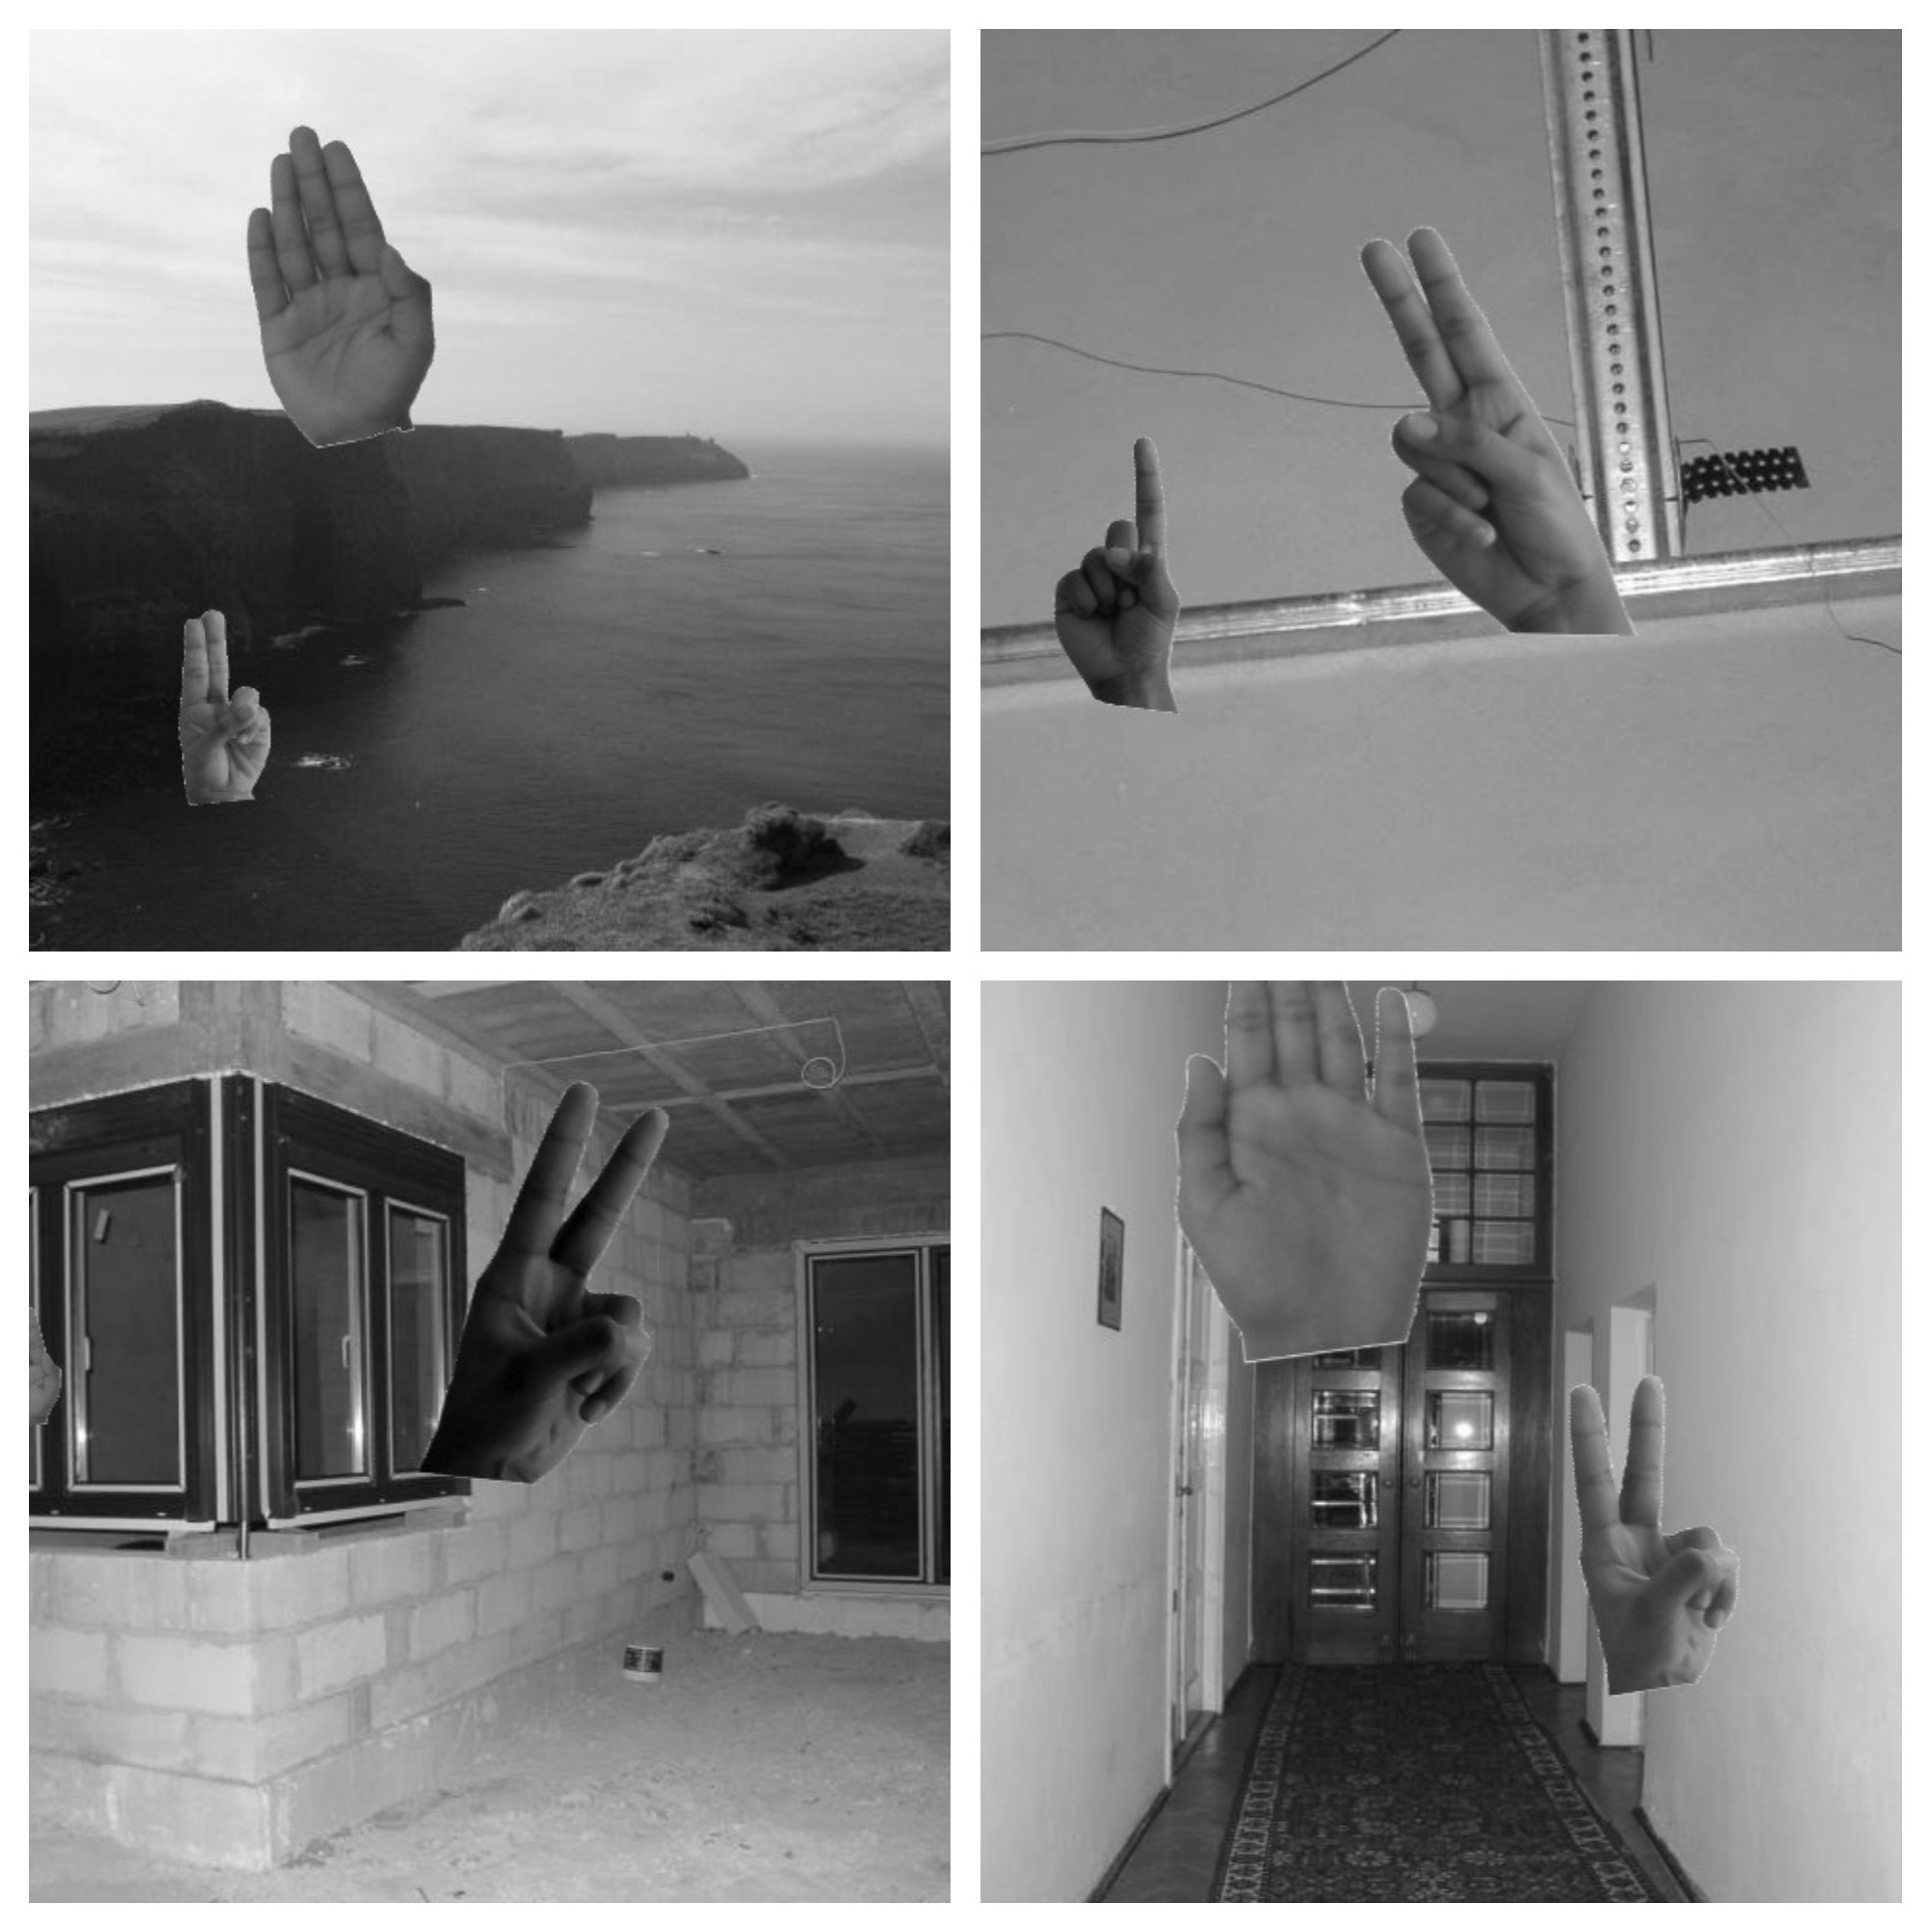
\includegraphics[width=8cm,height=4cm,angle=0]{positive_aug}
\end{figure}
\item \textit{Vectors:} All the positive descriptor files are concatenated into one file and then the \textit{cv\_createsamples} function is called again with the positive descriptor file and number of samples to generate as input which generates the vector file for the training process. The vector file contains all the information about the number of samples, what negatives were used, the size of the detector windows etc. The number of samples to be generated should be a multiple of 24.
\item \textit{Training:} The command \textit{cv\_traincascade} is called to train the cascade classifier using the previously collected vector file and the negative descriptor file. We also need to specify the number of positive and negative samples to use, although they should be less than the total amount present as the trainer consumes more samples than we specify. The detector size should be the same throughout and should always be a multiple of 24.
\item \textit{Log outputs:}
[image of log]
\par [explain the log prints of the training process]
\end{enumerate} 
The following algorithm succinctly sums up the entire training process:
\begin{algorithm}[H]
\caption{Cascade Training}
\begin{algorithmic}[1]
\STATE $P \gets$ Precursor Set for Each Gesture
\STATE $R\gets$ Set of Negative Images
\STATE $N\gets$ Number of Positives To Generate for a Precursor
\STATE $W,H \gets$ Width and Height of Detector
\STATE $N_{vec}\gets$ Number of Vectors to Generate
\STATE $N_{pos},N_{neg}$ Number of Positive and Negative for Training
  \FORALL{$p \in P$}
  	\FORALL{$i \in p$}
	\STATE $i_{pos}\gets$ Set of $N$ Positive Images of $i$ Generated from $R$
	\STATE $i_{desc}\gets$ Descriptor of $i_{pos}$
	\STATE $p_{desc}\gets p_{desc}\mid i_{desc}$  
	\ENDFOR
  \STATE $p_{vec}\gets$ Vectorize $p_{desc}$ with $N_{vec}$
  \STATE $cascade\gets$ Train on $p_{vec}$ with $N_{pos}$, $N_{neg}$, $W$ and $H$
  \ENDFOR
\end{algorithmic}
\end{algorithm}

Finally, we have three different Haar cascade classifiers that can detect each type of gesture. These are stored as \textit{.xml} files which can be imported into python and used to detect the relevant gestures.

\subsection{Visualization}
The \textit{Cascade Detectors} return coordinates of the detected objects which can be used for visualization.
\par There are a few tunable parameters that help in improving the recognition task and eliminating False Positives:
\begin{enumerate}
\item \textit{Neighbors}: The minimum number of neighbors for a detection window to be classified as positive.
\item \textit{Window}: The Window of Detection. Does not have a huge impact but ideal for setting up ROI.
\end{enumerate}
\begin{enumerate}
\item \textit{Bounding Boxes:} The return values of the classifier are used to draw bounding boxes around the detected objects. An ideal detector would just return one object which is the hand gesture.
[image of boxes of all detectors]
\item \textit{Convex Hull:} The detected gesture ROI is then used to draw a convex hull around the contours of the gesture. The ROI prevents spurious contours to be detected as the convex hull gets fit on the contour with the highest area.
[image of a convex hull]
\item \textit{Defects:} Defects are the points of the contour which are furthest from the fitted hull. This can be used to detect how many fingers were put up as the number of defects is always one less than the number of open fingers. Since we already detected the appropriate gesture using different classifiers, this step is can be used to fine tune the detector.
\item \textit{Interface Actions:} The detected gestures perform specific actions. The challenge would be to break off the detection once the action is performed in order to prevent the same action from being executed in a loop.
\end{enumerate}
The Algorithm below summarizes the detection stage for each image frame:
\begin{algorithm}[H]
\caption{Gesture Detection}
\begin{algorithmic}[1]
\STATE $C \gets$ Set of Cascade Detectors
\STATE $I$ Image Frame
\STATE $P$ Set of Parameters for Each Detector
  \FORALL{$c \in C \and p \in P$}
	\STATE $w \gets$ Run $c$ on $I$ subject to $p$
	\STATE $I_{roi}\gets$ Subset $I$ with $w$
	\STATE $I_{b}\gets$ Threshold and Binarize $I_{roi}$
	\STATE $I_{h}\gets$ Convex Hull of $i_b$
	\STATE $I\gets$  Overly $I_h$ on $I$ 
  \ENDFOR
\end{algorithmic}
\end{algorithm}
The performance of the detector is discussed in the next section.
\section{Results and Conclusion}
[talk about performance, training times as well as the challenges faced and the shortcomings of the program]
As mentioned before, one Haar Cascade Classifier was trained for each of the three gestures and the two finger gesture was re-trained using augmented negative images as the false positive rate was high and the classifier was recognizing other gestures as well. Out of the approximate 30 precursor images for each gesture, 15 were randomly selected for training.
\par Instead of training the classifiers for the entire 20 stages, the training was stopped when a lower limit of $10^{-4}$ for the \textit{Acceptance Ratio} to prevent over-fitting. The \textit{False Alarm Rate} was set to $0.5$ and provided decent results while keeping training time low within 30 minutes. The low training time is partly due to the low FA rate as well as other factors such as higher RAM availability, high CPU clock rate, smaller window size of detector, low number of training samples to name a few.
\par The classifiers were trained on a machine running MacOS Sierra 10.12.6 with a \textit{Quad Code CPU @ 4.4 GHz} and \textit{16 Gb 3000 MHz DDR4 RAM}.
\par The following table summarizes the training:
\begin{table}[H]
\centering
\caption{Training Data}
\begin{tabular}{|c|c|c|c|c|c|}
\hline
\bfseries Gesture &\bfseries Samples & \bfseries Positive & \bfseries Negative & \bfseries Stages\\
\hline
Palm & 1920 & 1700 & 900 & 11\\
1 Finger & 1920 & 1700 & 900 & 13\\
2 Fingers & 1920 & 1700 & 900 & 13\\
2 Fingers (Aug.) & 3840 & 3600 & 1900 & 12\\
\hline
\end{tabular}
\end{table}
%% You Can make changes below this
%%=============================================================================================================================================================================
\begin{figure}[H]
\centering
\caption{Palm Detector}
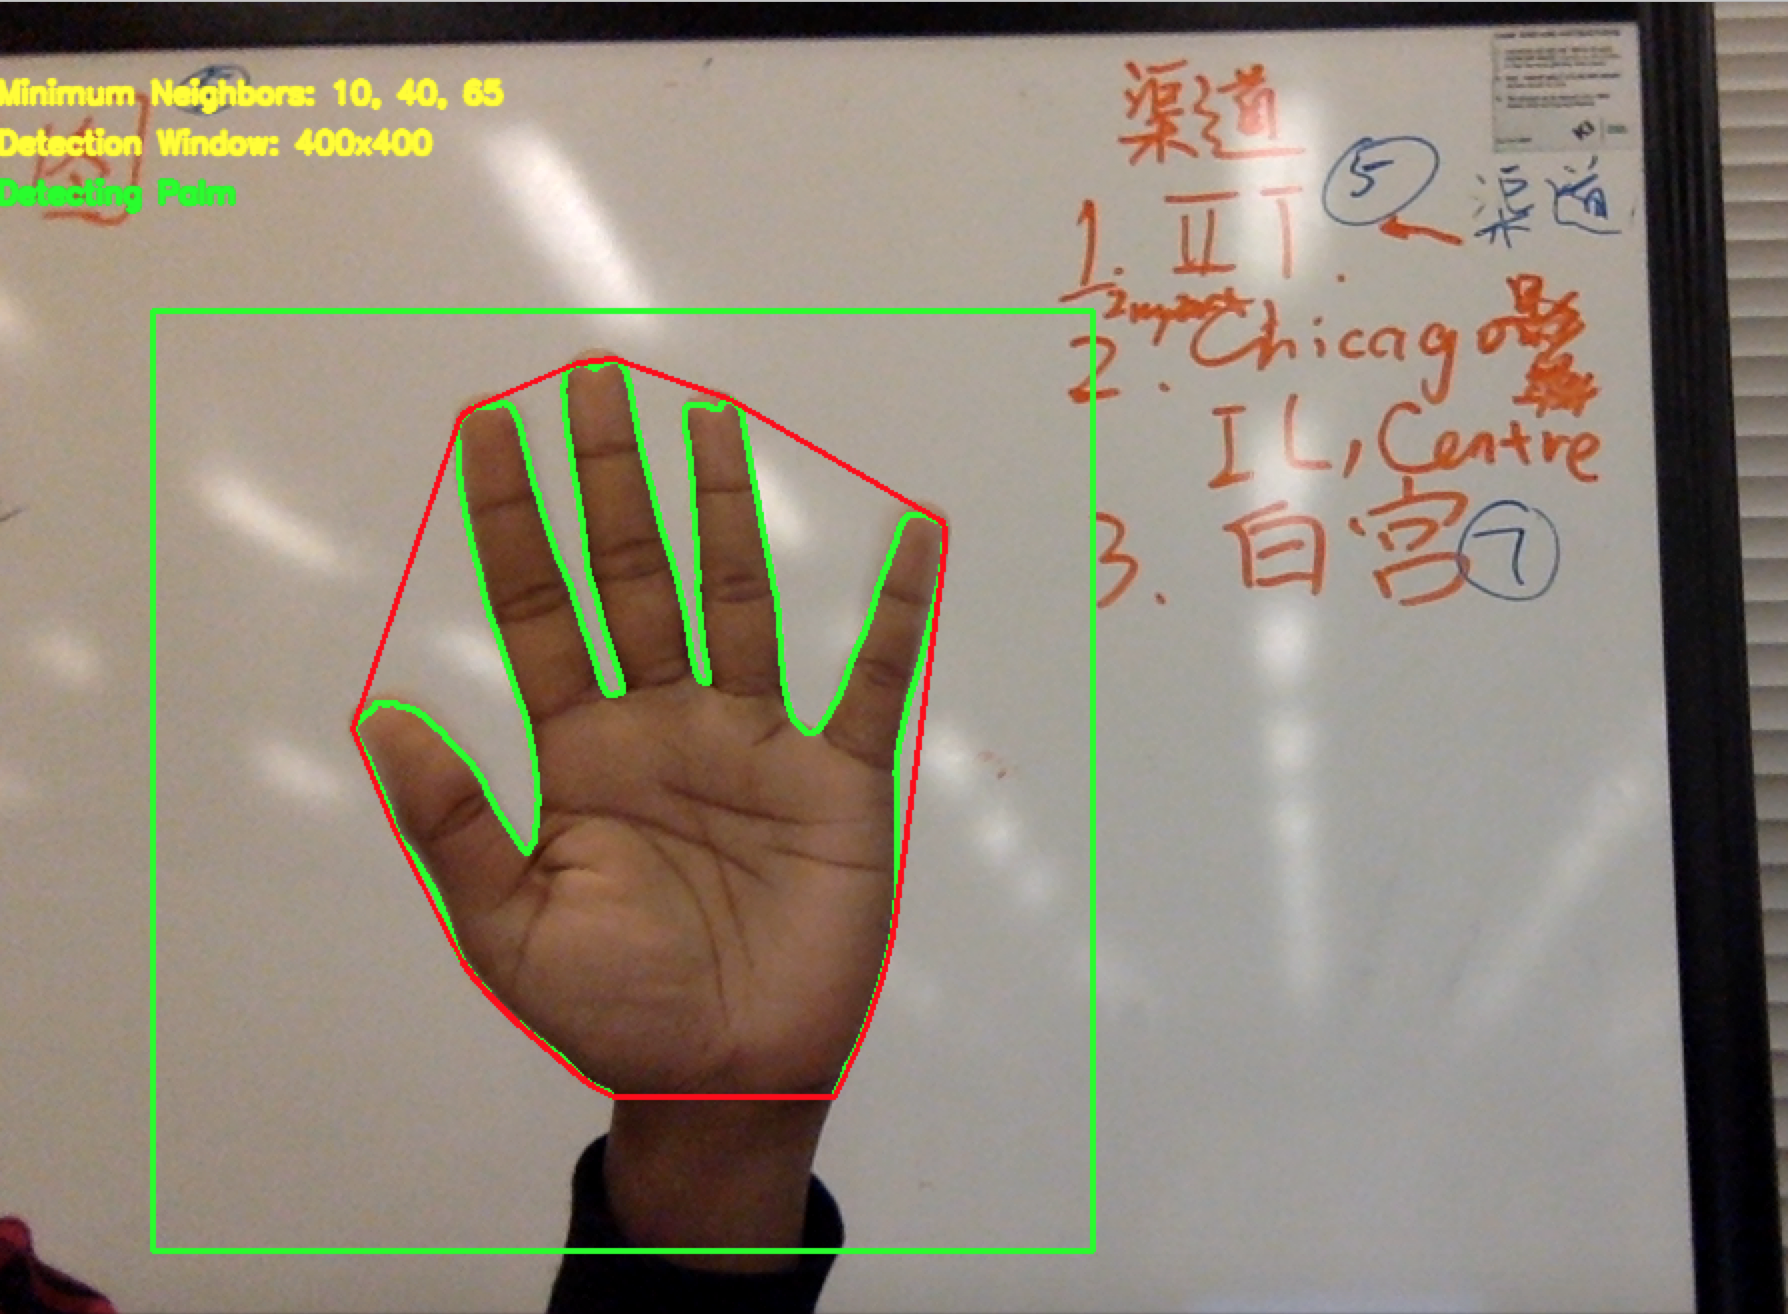
\includegraphics[width=8cm,height=4cm,angle=0]{palm1}
\end{figure}

The detector was tested on 100 images each of palm, one finger and two finger gestures. The results are summarized in the table below.
\begin{table}[H]
\centering
\caption{Performance}
\begin{tabular}{|c|c|c|c|}
\hline
\bfseries Gesture &\bfseries FP & \bfseries FN & \bfseries Accuracy\\
\hline
Palm & - & - & -\\
1 Finger & - & - & -\\
2 Fingers & - & - & -\\
2 Fingers (Aug.) & - & - & -\\
\hline
\end{tabular}
\end{table}

The major concern was between the erroneous detections of the one-finger and two-finger detectors as two fingers joined together were being detected as a single finger. This can be fixed by increasing the training sample size and reducing the False alarm rate. Note that an FA of 0.5 performed decently as decreasing the FA would exponentially increase the training time (A highly accurate Haar Cascade takes weeks to train).
\par
In essence, the gesture detector's performance was satisfactory considering the short training time and small sample size.

\begin{thebibliography}{9}

\bibitem{main1}
  Ruchi Manish Gurav and Premanand K. Kadbe,
  \textit{Real time Finger Tracking and Contour Detection for Gesture Recognition using OpenCV},
  2015 International Conference on Industrial Instrumentation and Control (ICIC).

\bibitem{haar1}
  Qing Chen Nicolas, D. Georganas, and Emil M. Petriu,
  \textit{Hand Gesture Recognition Using Haar-Like Features And A Stochastic Context-Free Grammar},
   IEEE ,Vol. 57, No. 8, August 2008.

\bibitem{skindet1}
  Amit Kumar and Shivani Malhotra ,
  \textit{Real-time human skin color detection algorithm using skin color map},
  2015 2nd International Conference on Computing for Sustainable Global Development (INDIACom), 
  2015, 
  p2002 - 2006

\bibitem{backsub1}
  Lianqiang Niu and Nan Jiang,
  \textit{A Moving Objects Detection Algorithm Based on Improved Background Subtraction},
  2008 Eighth International Conference on Intelligent Systems Design and Applications, 
  2008, 
  Vol. 3, 
  p604 - 607
\end{thebibliography}

\end{document}
